%
% This file is part of RHexLib, 
%
% Copyright (c) 2001 The University of Michigan, its Regents,
% Fellows, Employees and Agents. All rights reserved, and distributed as
% free software under the following license.
% 
%  Redistribution and use in source and binary forms, with or without
% modification, are permitted provided that the following conditions are
% met:
% 
% 1) Redistributions of source code must retain the above copyright
% notice, this list of conditions, the following disclaimer and the
% file called "CREDITS" which accompanies this distribution.
% 
% 2) Redistributions in binary form must reproduce the above copyright
% notice, this list of conditions, the following disclaimer and the file
% called "CREDITS" which accompanies this distribution in the
% documentation and/or other materials provided with the distribution.
% 
% 3) Neither the name of the University of Michigan, Ann Arbor or the
% names of its contributors may be used to endorse or promote products
% derived from this software without specific prior written permission.
% 
% THIS SOFTWARE IS PROVIDED BY THE COPYRIGHT HOLDERS AND CONTRIBUTORS
% "AS IS" AND ANY EXPRESS OR IMPLIED WARRANTIES, INCLUDING, BUT NOT
% LIMITED TO, THE IMPLIED WARRANTIES OF MERCHANTABILITY AND FITNESS FOR
% A PARTICULAR PURPOSE ARE DISCLAIMED. IN NO EVENT SHALL THE REGENTS OR
% CONTRIBUTORS BE LIABLE FOR ANY DIRECT, INDIRECT, INCIDENTAL, SPECIAL,
% EXEMPLARY, OR CONSEQUENTIAL DAMAGES (INCLUDING, BUT NOT LIMITED TO,
% PROCUREMENT OF SUBSTITUTE GOODS OR SERVICES; LOSS OF USE, DATA, OR
% PROFITS; OR BUSINESS INTERRUPTION) HOWEVER CAUSED AND ON ANY THEORY OF
% LIABILITY, WHETHER IN CONTRACT, STRICT LIABILITY, OR TORT (INCLUDING
% NEGLIGENCE OR OTHERWISE) ARISING IN ANY WAY OUT OF THE USE OF THIS
% SOFTWARE, EVEN IF ADVISED OF THE POSSIBILITY OF SUCH DAMAGE.

%%%%%%%%%%%%%%%%%%%%%%%%%%%%%%%%%%%%%%%%%%%%%%%%%%%%%%%%%%%%%%%%%%%%%%
% $Id: quickstart.tex,v 1.12 2001/07/20 00:41:11 ulucs Exp $
%
% Created       : Uluc Saranli, 01/06/2001
% Last Modified : Uluc Saranli, 06/27/2001
%
%%%%%%%%%%%%%%%%%%%%%%%%%%%%%%%%%%%%%%%%%%%%%%%%%%%%%%%%%%%%%%%%%%%%%%

\chapter{Quick Start Tutorial}
\label{sec:quickstart}

\section{Library Installation}

This section describes the basic procedures for installing and configuring
RHexLib and the optional simulation components SimSect++ and Geomview. The
latest version of RHexLib and SimSect++ can be downloaded from {\tt
http://ai.eecs.umich.edu/RHex/Internal/RHexLibdetails.html}. Geomview can be
downloaded from {\tt http://geom.umn.edu}.

\subsection{System Requirements}

The current version of RHexLib works with both the Linux and QNX operating
systems. The Linux version requires the use of either the {\em virtual} or
{\em SimSect} hardware libraries to provide a simulated interface to the low
level functionality of RHex. The QNX version does not work with the SimSect
hardware library.

The current version of SimSect++ works only with Linux as it requires the
use of Geomview (which is only available under Unix) for visualization.

Geomview currently works only with Unix-like platforms. Please refer to {\tt
http://www.geomview.org} for information about development of this
visualization tool.

\subsection{Installing SimSect++}

\begin{itemize}
\item{{\bf Create the directory structure}

Create a directory {\tt RHex}, where RHexLib, SimSect++ and all the user
development directories will reside:

{\tt 
mkdir RHex \\
cd RHex
}}

\item{{\bf Uncompress the library distribution}

Under the directory {\tt RHex}, uncompress SimSect++.tar.gz with the
following commands:

{\tt
gzip -d ../SimSect++.tar.gz\\
tar -xvf ../SimSect++.tar
}

This will create a directory called {\tt SimSect++}, where the library
distribution will reside.}

\item{{\bf Configure environment variables}

If you are using {\tt tcsh} as your Unix shell, add the following lines to
the {\tt .cshrc} file in your home directory:

{\tt
setenv SIMSECT\_DIR \~{}/RHex/SimSect++
}

Also, execute this command in your current shell so that they immediately
take effect.

Similarly, if you are using {\tt bash} as your Unix shell, add the following
lines to your {\tt .bashrc} file in your home directory:

{\tt
export SIMSECT\_DIR=\~{}/RHex/SimSect++
}}

\item{{\bf Compile the library}

Compile the library using the following commands from within the SimSect++
directory:

{\tt
make depend \\
make clean \\
make
}

This will compile and create the SimSect++ integration engine and model
libraries and place links to them in {\tt SimSect++/lib}. Moreover, it will
also create a standalone SimSect hexapod model simulation executable in {\tt
SimSect++/bin} }.

\end{itemize}

\subsection{Installing Geomview}

Please refer to Geomview installation instructions in {\tt
  http://geom.umn.edu}.

\subsection{Installing RHexLib under Linux}

\begin{itemize}
\item{{\bf Create the directory structure}

Create a directory called {\tt RHex}, where RHexLib, SimSect++ and all the
user development directories will reside. Note that if you already installed
SimSect++, you will already have created this directory.

{\tt 
mkdir RHex \\
cd RHex
}}

\item{{\bf Uncompress the library distribution}

In the directory {\tt RHex}, uncompress RHexLib.tar.gz with the
following commands:

{\tt
gzip -d ../RHexLib.tar.gz\\
tar -xvf ../RHexLib.tar
}

This will create a directory called {\tt RHexLib}, where the library
distribution will reside.}

\item{{\bf Configure environment variables}

If you are using {\tt tcsh} as your Unix shell, add the following lines to
the {\tt .cshrc} file in your home directory:

{\tt
setenv RHEX\_DIR \~{}/RHex/RHexLib\\
setenv RHEX\_HARDWARE \_MICHIGAN\_
}

Also, execute these commands in your current shell so that they immediately
take effect.

Note that setting {\tt RHEX\_HARDWARE} to either {\tt \_MICHIGAN\_} or {\tt
\_MCGILL\_} will determine which hardware configuration will be used for the
example files in the library.

Similarly, if you are using {\tt bash} as your Unix shell, add the following
lines to your {\tt .bashrc} file in your home directory:

{\tt
export RHEX\_DIR=\~{}/RHex/RHexLib\\
export RHEX\_HARDWARE=\_MICHIGAN\_
}}

\item{{\bf Compile the library}

Compile the library using the following commands:

{\tt
make depend \\
make clean \\
make all
}

This will compile and create the RHexLib core and hardware libraries and
place links to them in {\tt RHexLib/lib}. Moreover, it will also create
example executables in {\tt RHexLib/examples} }.

\end{itemize}

\subsection{Installing RHexLib under QNX}

The installation procedure under QNX is identical to the Linux installation
procedures of the preceding section. QNX will most likely have a bash-like
shell to start with, so use the bash specific instructions.

It is recommended that you create a specific user called {\tt rhex} and do
all the library compilation as that user rather than as the {\tt root}
user. Even though the executables will need to run as root to access
privileged IO instructions, development and compilation can (and should)
proceed without root privileges.

\subsection{Working with the Libraries} \label{sec:worklibraries}

RHexLib is designed to be a modular library, where users that need to create
controllers and design modules should not need to change any of the library
code. Consequently, instead of working in the library
distribution directory, each programmer should create a directory tree of
their own to do development. For example, a typical directory for the {\tt
  rhex} user on the robot would look like:\\

{\tt 
\noindent\~{}rhex \\
\~{}rhex/RHex \\
\~{}rhex/RHex/RHexLib \\
\~{}rhex/RHex/SimSect++ \\
\~{}rhex/RHex/UlucDevel \\
\~{}rhex/RHex/EricDevel
...
}\\

Developers should copy example files from {\tt RHexLib/examples} to their
own directory before making any changes or testing their controllers.

The directory {\tt RHexLib/tools} contains an example makefile called {\tt
Makefile.sample} to be used for compiling programs that use RHexLib. Users
can copy this file to their development directory and edit it to compile
their controllers:

{\tt 
\noindent cp RHexLib/tools/Makefile.sample UlucDevel/Makefile \\
}

You will need to make the following changes in the makefile before you can
compile programs:\\

{\tt
\noindent EXEC = example
}\\

This line specifies the name of the executable program that the compiler
will generate. The RHexLib makefile tools also expect to find a file with
the same base name and a {\tt .cc} extension in the same directory ({\tt
  example.cc}, in this case). Normally, this file is where {\tt main()} will 
be defined.\\

{\tt
\noindent SOURCES = SampleModule.cc ControlMachine.cc
}\\

This line specifies source files containing additional module, controller
and utilitie definitions that the user wants to link to the main
executable. It is always a good practice to separate components in the
controllers such as state machines, modules etc. into separate files and
specify them in the {\tt SOURCES} line. It will speed up compilation and
make it easier to navigate through your code.

If your sources require additional flags, they can be configured with an
additional line in the Makefile.\\

{\tt
\noindent AUXFLAGS = -I~rhex/RHex/UlucDevel/include
}\\

The RHexLib libraries that are required by your source must be included in
an additional statement. For example, for compilation on the Michigan RHex
the following line would need to be included in the Makefile.\\

{\tt
\noindent LIBS = librhex.a libmichiganhw.a libcommonhw.a libbase.a
}\\

Note that the order in which these libraries are specified is usually
important and can lead to compilation errors if not done properly. If
libraries which are not part of RHexLib (such as SimSect++ libraries {\tt
  libhexapod.a} {\tt libengine.a}), are to be linked, they must be indicated
in another statement as well.\\

{\tt
\noindent AUXLIBS = libhexapod.a libengine.a
}\\

Once {\tt Makefile} is modified appropriately, commands similar to the
following will create an executable.\\

{\tt
\noindent cd UlucDevel \\
make depend \\
make clean \\
make
}\\

Note that this sequence of commands deletes all precompiled object files,
and recompiles everything. In cases where small modifications are made to
the source files, the following command will be sufficient:\\

{\tt
\noindent make
}\\

\section{Basic Module Example: PrintModule}

This section describes the details of implementing a simple RHexLib program
which periodically displays the encoder counters. A similar example, {\tt
enc\_test\_mm}, can be found in the {\tt examples} directory of the source
distribution.

\subsection{The {\tt PrintModule} Class}

In RHexLib, any task that needs to be performed periodically is defined as 
a {\em Module}, more specifically as a class derived from the {\tt Module}
abstract base class. Below is a definition of the {\tt PrintModule} class,
which encapsulates the task of periodically reading and printing the encoder 
counter values.

\begin{codesegment}
#include "Hardware.hh"

class PrintModule : public Module {

public:
  PrintModule ( void ) : Module( "print", 0, false, false ) { };

  void init( void );
  void uninit( void ) { };
  void activate( void );
  void deactivate( void );
  void update( void );

private:
  Hardware *hardware;
};
\end{codesegment}

Note that each class derived from the virtual base class {\tt Module} must
define five methods: {\tt init()}, {\tt uninit()}, {\tt activate()}, {\tt
deactivate()} and {\tt update()}. These methods provide a a standard
interface to the {\tt ModuleManager} which, among other tasks, keeps a list
of all modules, manages their states, and calls the above methods at
appropriate times. In the case of {\tt PrintModule}, the {\tt uninit()}
method does not do anything, the rest of the methods are defined below.

An important detail to note is that the {\tt Module} class constructor takes
four arguments. The first two determine the {\em name} and {\em index} of
the module, which are used together to uniquely identify each module in the
system. The last two arguments determine the {\em type} of the module and
are explained in later chapters of this manual.

\subsection{The {\tt init()} method}

The {\tt init()} method of a module is called whenever the module is added
to the module manager's list with a call to the function {\tt
MMAddModule()}. The {\tt init} method is usually responsible for
initializing related hardware components and finding components and other
modules that are needed for the module's operation. In our example, the {\tt
PrintModule}, we will need access to the low level hardware interface, so
initialization involves acquiring a pointer to the interface object.

\begin{codesegment}
void PrintModule::init( void ) {
  hardware = MMGetHardware();
}
\end{codesegment}

The {\tt MMGetHardware()} function call returns a pointer to the currently
selected hardware interface object for the module manager. The selection of
this object usually takes place in {\tt main()} with a call to the function
{\tt MMChooseHardware()}.

\subsection{The {\tt activate()} method}

The {\tt activate()} method of a module is called whenever the module is
activated by the module manager via a call to either {\tt
MMActivateModule()} or the first call to {\tt MMGrabModule()}. This changes
the the module from the {\tt INACTIVE} state to the {\tt ACTIVE} state,
which means that the module manager will begin to periodically call the {\tt
update()} method of the module.

Activating a module usually involves making sure that all the components
needed for the task are active and operational. Moreover, necessary
initializations of the components must also be performed. For our example,
the {\tt PrintModule} will enable all the encoders using the hardware
interface.

\begin{codesegment}
void PrintModule::activate( void ) {
  int axis;

  for ( axis = 0; axis < 6; axis++ )
    hardware->encoders->enable( axis );
}
\end{codesegment}

\subsection{The {\tt deactivate()} method}

The {\tt deactivate()} method of a module is called whenever the module is
deactivated through a call to either {\tt MMDeactivateModule()} or the last
call to {\tt MMReleaseModule()}. This puts the module in the {\tt INACTIVE}
state, which means that the {\tt update()} method of the module will not be
called anymore.

For our example, upon deactivation, the {\tt PrintModule} will disable all
the encoders using the hardware interface.

\begin{codesegment}
void PrintModule::deactivate( void ) {
  int axis;

  for ( axis = 0; axis < 6; axis++ )
    hardware->encoders->disable( axis );
}
\end{codesegment}

\subsection{The {\tt update()} method}

The {\tt update()} method of a module is where its core functionality is
defined. When a module is in the {\tt ACTIVE} state, its {\tt update()}
function is called periodically by the module manager.

Our example module, the {\tt PrintModule}, will read the encoders and print
their contents in its {\tt update()} method. Moreover, it will also be
responsible for detecting keyboard input and exiting the program.

\begin{codesegment}
void  PrintModule::update ( void ) {
  int axis;

  printf( "Encoders: " );

  for ( axis = 0; axis < 6; axis++ )
    printf( "0x%04x, ", hw.encoders->read( axis ) );

  printf( "\n" );

  if ( kbhit() ) {
    MMMessage( "User interrupt: Shutting down!\n" );
    MMPowerOff( );speedd-speed
  }
}
\end{codesegment}

\section{Using PrintModule in a program}
 \label{sec:together}

What makes modules operational in RHexLib is the {\em Module Manager}. In
order to be operational, modules must be created as instatiations of the
class, and the module manager must be informed of its presence through the
{\tt MMAddModule()} library call. Moreover, it needs to be activated through
the {\tt MMActivateModule()} or {\tt MMGrabModule()} library functions in
order for its update() function to start being called periodically.

The library function {\tt MMMainLoop()} is the main entry point to the
module manager, and it never returns. It is usually called once from main(),
after all the desired modules are created and added to the module manager's
list. Once this function is called, the module manager takes control and
handles the periodic issues of module updates as well as other timing tasks.
Following a call to {\tt MMMainLoop()}, the only way to exit the program is
through the {\tt MMPowerOff()} function, from within one of the module
methods.

As such, there is a very typical way in which RHexLib programs are
built. The following program is the main entry point to our small example
and demonstrates how things are setup in a typical RHexLib program..
 
\begin{codesegment}

#include "ModuleManager.hh"
#include "SimSectHW.hh"

SimSectHW hw; // Create an instance of the SimSect hardware object.

int main( void ) {

  PrintModule pr; // Create an instance of the PrintModule module.

  // Let the module manager know about the current hardware
  MMChooseHardware( &hw );

  // Add and activate the print module
  MMAddModule( &pr, 10, 0, 10 );
  MMActivateModule( &pr );

  // Call the Module Manager main loop
  MMMainLoop();

  // Normally, the MMMainLoop() does not exit, so this point is never reached.
  return 0;
}
\end{codesegment}

As this code segment shows, the typical structure of {\tt main()} is as
follows:
\begin{itemize}
\item{Create an instance of the desired Hardware object}
\item{Call {\tt MMChooseHardware()} to inform the module manager the pointer
    to the hardware object.}
\item{Create and initialize all modules that will be used by the program.}
\item{Add the newly created modules to the module manager's list through
    {\tt MMAddModule()} function calls.}
\item{Activate the necessary modules through {\tt MMActivateModule()}
    function calls}
\item{Call {\tt MMMainLoop()}}
\end{itemize}

From then on, the module methods will determine the flow of the
execution. Note that at least one module needs to be activated before {\tt
MMMainLoop()} is called. Otherwise, the program will be stuck in an infinite
loop, and no module updates will take place.

An important detail is that the parameters of a module related to the
scheduling of its updates are determined by the {\tt MMAddModule( Module *,
  int period, int offset, int order )} function
call. It is hence possible to configure the {\em period}, the starting time
{\em offset} and the update {\em order} (in case of multiple updates
scheduled at the same time) of each module.

\section{Basic Controller Example: PushupController} \label{sec-pushup}

In this section we describe a more complicated module: a RHex-specific
controller which controls the robot to continuously do ``pushups''. It
demonstrates the simplest way of building a controller in RHexLib, how basic
motor control tasks are accomplished. It also shows some of the
configuration facilities commonly used in RHexLib.

This controller assumes that RHex is in the standing position to start
with. Starting there, it brings all the legs to a vertical position (making
the robot sit), waits there for a moment, and then stands up again,
restarting the cycle.

\subsection{The Module Definition}

Here we describe the details of how to define the {\tt PushupController}
module class and explain some of the components required by this
controller. Usually, the definitions of module classes in RHexLib are done
in separate header files, defining the interface of the module with the rest
of the library. In this case, the class definition will reside in {\tt
PushupController.hh}.

\begin{codesegment}
#include "ModuleManager.hh"
#include "PositionControl.hh"
#include "Profiler.hh"

class PushupController : public Module {

public:
  PushupController ( void )
    : Module( "pushupcontroller", 0, true, false ) { };

  // Module base class interface
  void  init ( void );
  void  uninit ( void ) { };
  void  activate ( void );
  void  deactivate ( void );
  void  update ( void );
\end{codesegment}

This part of the class definition is straightforward. We simply define the
standard module functions in a way similar to the previous example, the {\tt
PrintModule}. Once again, the name and index of the module are determined in
the definition of the class constructor, through the instatiation of the
base class {\tt Module}. Note also that in this case, all the module
functions except the uninit() method will be defined in the implementation
file {\tt PushupController.cc}.

Next we define a few private variables nad methods, local to {\tt
PushupController}.

\begin{codesegment}
private:

  PositionControl *control[6];
\end{codesegment}

These member variables will be pointers to the six different position
controller modules, associated with each one of the six legs. {\tt
PositionControl} modules implement basic proportional derivative(PD) control
feedback for all the motors in the system. Through their public interface,
our controller will be able to set the target positions for each leg,
updated every millisecond, commanding the legs perform the desired actions.

\begin{codesegment}
  MotorGains_t     oldGains[6];
\end{codesegment}

These member variables hold the PD gains that may have been in use by the
position controllers before the pushup controller is activated. When the
controller is deactivated, it will restore these gains to leave the position
controllers in their previous state. This is usually a good practice because
other components in the system might be expecting the PD gains to remain
unchanged for proper operation.

\begin{codesegment}
  Profiler         legProfiler;
\end{codesegment}

This member variable instantiates a {\tt Profiler} object, which is
responsible from generating the leg position as a function of time, also
called leg profile. Note that we only have one such object because, for the
pushup controller, all the legs are synchronized. Cconsequently, the desired
positions for all six legs will be the same at all times.

In RHexLib, the actual PD control of the leg motors and the generation of
the associated position profile are performed separately. Every millisecond,
our controller will ask the leg profiler the desired position for all the
legs. Then, it will set this new target on all six position
controllers. This scheme abstracts the generation of the desired leg
trajectories from the local PD feedback loop on the leg motors.

\begin{codesegment}
  void trackCurrentProfile( void );
\end{codesegment}

This utility method provides a facility to read the current value of the leg 
profiler and inform all the motor position controllers about the new target.

\begin{codesegment}
  double lowerTime;  // Time in seconds to lower the robot
  double chillTime;  // Time in seconds to chill, sitting down
  double standTime;  // Time in seconds to raise the robot up
  double waitTime;   // Time in seconds to wait standing up.
\end{codesegment}

These member variables determine how much time the controller should spend
in each of its stages. The pushup behavior can be decomposed into four
stages: lowering, chilling after sitting down, standing up and waiting in a
standing position. These variables determine how much time is spent in each
of these stages.

\begin{codesegment}
  int phase;
\end{codesegment}

This member variable indicates the current discrete ``phase'' of the
controllers. In implementing the aforementioned four different stages, the
pushup controller goes through six phases, where the controller actions are
defined as follows:

\begin{center}
\begin{tabular}{l}
0 : Starting to lower the robot \\
1 : Waiting for the robot to lower \\
2 : Wait for a while in the sitting position \\
3 : Starting to standup \\
4 : Waiting for the robot to standup \\
5 : Wait for a while in the standing position
\end{tabular}
\end{center}

Another way to write this controller is to use the {\tt StateMachine}
facilites of RHexLib. For this relatively simple example, we do not need the
power of state machines. If there were many more than six states, or if the
states were not visited in a simple cycle, or if the events that trigger
state transitions are were not so simple, state machines would probably make
the task simpler. {\tt StateMachine}s are covered later in this chapter and
elsewhere in this manual.

\begin{codesegment}
  double mark;
};
\end{codesegment}

This member variable is used to hold the state time of each phase in order
to switch to the next phase at appropriate times, determined by the values
of the timing member variables described above.

\subsection{The {\tt init()} Method}

There are two tasks usually performed by the {\tt init()} method of modules:
1) locate other modules that are going to be used; and 2) initialize member
variables by reading configuration information from a resource file..

With the function {\tt MMFindModule()}, RHexLib provides a means to acquire
a pointer to other module objects in the system. Almost all the
functionality of the library is implemented with modules, including low
level motor control, higher level behaviors such as walking, standing,
sitting, pronking as well as utilities such as logging data. Normally, in
{\tt main()}, all such modules to be used by an executable program are
``added'' to the system through calls to {\tt MMAddModule()}. The module
manager thus has a list of all these components, and can find modules by
their name and index, which are two of the parameters to the {\tt
MMFindModule()} function.

\begin{codesegment}
void PushupController::init( void ) {
  int i;

  for ( i = 0; i < 6; i ++ ) {
    if ( ( control[i] = ( PositionControl * ) 
           MMFindModule( POSITIONCONTROL_NAME, i )) == NULL)
      MMFatalError ( "PushupController::init", 
                     "Cannot find motor controller!" );
  }
\end{codesegment}

This part of the init method locates all six {\tt PositionControl}
modules. All of these six modules have the same name, defined in {\tt
StdModules.hh} as the macro {\tt POSITIONCONTROL\_NAME}, and their index
identifies which motor axis they correspond to. If {\tt MMFindModule()}
function call returns {\tt NULL}, indicating that the required module has
not yet been added to the module manager's list, a fatal error is generated,
and the program exits.

\begin{codesegment}
  lowerTime = MMGetFloatSymbol( "pushup_lower_time" , 1.0 );
  chillTime = MMGetFloatSymbol( "pushup_chill_time" , 0.3 );
  standTime = MMGetFloatSymbol( "pushup_stand_time" , 0.4 );
  waitTime = MMGetFloatSymbol( "pushup_wait_time" , 0.3 );
}
\end{codesegment}

The second part of the init method initializes the timing configuration of
the pushup machine. RHexLib maintains a global symbol table, where symbol
names are associated with either a floating point or a string value. Modules
in the system can access the table using {\tt MMGetFloatSymbol()} and {\tt
MMGetStringSymbol()} to retrieve the value of a particular symbol. These
functions also take a default value as an argument, to be returned if the
requested symbol cannot be found.

Usually, the symbol table is initialized by loading a ``configuration file''
using the {\tt MMReadConfig()} function in {\tt main()}. This configuration
file includes statements such as:

\begin{codesegment}
  pushup_lower_time = 0.9;
  pushup_chill_time = 0.2;
  pushup_stand_time = 0.5;
  pushup_wait_time = 0.2;
\end{codesegment}

which assign values to symbols. This mechanism provides means of
reconfiguring the behavior of controllers and modules without requiring that
the executable be recompiled.

\subsection{The {\tt activate()} Method}

The only modules used by the pushup controller are the motor position
controllers. Moreover, they are required throughout the whole operation of
the controller. As a consequence, the activate module method in this case is
responsible for requesting exclusive access to all six position controllers
and adjusting the PD gains appropriately.

\begin{codesegment}
void PushupController::activate( void ) {
  int          i;
  MotorGains_t gains;

  phase = 0;
\end{codesegment}

Every time the pushup controller is activated, it will start from phase 0:
starting to lower. The phase must be initialized in the activate method
because the same instantiation of this module may be activated more than
once (at different times) by different supervisory controllers.

\begin{codesegment}
  for ( i = 0; i < 6; i++ )
    MMGrabModule( control[i], this );
\end{codesegment}

This statement requests exclusive access to the motor position controller
modules whose pointers were acquired in the {\tt init} method. The functions
{\tt MMGrabModule()} and {\tt MMReleaseModule()} are thus used in pairs to
acquire and release the exclusive use of other modules in the system. They
should be used whenever the functionality of a module is needed to make sure
that the operation of other components in the system which might be using
the same modules is not disturbed.

In this context, there are two types of modules: {\tt SINGLE\_USER} and
{MULTI\_USER}. The type of a module is determined by its constructor. The
behavior of {\tt MMGrabModule()} is different for these two different types.

Single user modules can be grabbed by only one other module at a time. If a
second grab request is received, the system gives a fatal error and
exits. This mechanism makes sure that, for example, the motor position
controllers are not used by more than one entity at a time, which could
result in pretty chaotic behavior. Multi user modules can be grabbed as many
times as necessary.

Another feature of {\tt MMGrabModule()} is that the grabbed module
is also activated if it is not already active. Similarly, the {\tt
MMReleaseModule()} function deactivates the module if it has been
released as many times as it has been grabbed.  Hence, for multi user
modules, the first call to the grab function activates the module and the
last call to the release function deactivates the module.

\begin{codesegment}
  gains.kp = 5.0;
  gains.kd = 0.14;

  for ( i = 0; i < 6; i++ ) {
    control[i]->getGains( & oldGains[i] );
    control[i]->setGains( & gains );
  }
}
\end{codesegment}

This code segment saves the PD gains of the motor controllers and sets the
new gains to appropriate values for the pushup behavior.

\subsection{The {\tt deactivate()} Method}

The deactivate module method is usually responsible for releasing the
modules that have been grabbed in the activate method. In addition, it
usually restores their states to what they were before they were grabbed.

\begin{codesegment}
void PushupController::deactivate( void ) {
  int i;

  for ( i = 0; i < 6; i++ )
    control[i]->setGains( & oldGains[i] );
\end{codesegment}

This code segment restores the PD gains of the motor position controllers to 
their old values.

\begin{codesegment}
  for ( i = 0; i < 6; i++ )
    MMReleaseModule( control[i], this );
}
\end{codesegment}

Finally, all six motor position controllers are released to grant access to
anybody else who wants to use them.

\subsection{The {\tt update()} Method}

The update module method is where the bulk of the work is done for the
controller. All the other module methods are mainly for initialization and
clean integration with the rest of the system and do not much else.

Depending on the current phase of the controller, the update method, being
called once every millisecond, has to perform different tasks. As a
consequence, it ends up being a big case statement, implementing a primitive
state machine which linearly proceeds through 6 states (or phases). In later
sections, we will see more structured and formal ways of defining state
machines, which will allow the programmer to define much more complex
behaviors. Beyond 5 or 6 states, with transitions depending on events other
than simple timers, defining state machines through case statements quickly
becomes unelegant.

\begin{codesegment}
void PushupController::update( void ) {

  int           i;
  MotorTarget_t target;
  double        now = MMReadTime();
\end{codesegment}

This segment defines the local variables. An important function to note is
{\tt MMreadTime()}, which returns the current time in seconds.

\begin{codesegment}
  switch ( phase ) {
  case 0:   // Starting to lower the robot

    legProfiler.setup( SEC_TO_CLOCK(now), SEC_TO_CLOCK(now + lowerTime), 
                       0, M_PI / 2 );
\end{codesegment}

As described in the preceding sections, phase 0 in the pushup controller is
when the robot starts to lower. Hence, in this state, we initialize the leg
profile to bring the leg to a horizontal position and immediately proceed
with the next phase.

The {\tt setup(t1, t2, val2, val2)} method of the {\tt Profiler} class is
used to initialize a linear time trajectory for the leg between two angle
values. The resulting trajectory has the following functional form:

\begin{equation*}
f(t) = \left\{\begin{array}{l@{\hspace{0.3in}}l}
val_1 & t < t_1 \\
val_1 + {(t-t_1) (val_2-val_1)}/{t_2-t_1)} & t_1 \leq t \leq t_2 \\
val_2 & t > t_2 \\
\end{array}\right.
\end{equation*}

Note that this interface does not know anything about the $2 \pi$
periodicity of angles, and interprets $val_1$ and $val_2$ as real
numbers. The pushup controller, in order to lower the robot to the ground,
sets up a linear profile starting from 0 (vertical legs) and going to
$\pi/2$ (horizontal legs) in the amount of time configured in the init method.

\begin{codesegment}
    mark = now;
    phase = 1;
    break;
\end{codesegment}

This phase of execution also marks the current time to measure how much more 
the controller needs to wait before initiating the chilling phase. Also, the
assignment to the phase member variable transitions into phase 1, which
waits for the robot lowering to end.

\begin{codesegment}
  case 1:   // Waiting for the robot to lower

    if ( now < ( mark + lowerTime ) )
      trackCurrentProfile();
    else {
      mark = now;
      phase = 2;
    }
    break;
\end{codesegment}

During phase 1, the controller does not change the profile which has been
setup in phase 0. However, it reads the current target position from the
profile and commands the motors to go to the current target angle through
repeated calls to the {\tt trackCurrentProfile()} method (whose details are
explained later). When the legs reach their horizontal position
(i.e. when {\tt lowerTime} amount of time has elapsed), the controller
switches to phase 2.

\begin{codesegment}
  case 2:   // Wait for a while in the sitting position

    if ( now > ( mark + chillTime ) ) {
      mark = now;
      phase = 3;
    }
    break;
\end{codesegment}

During this phase, the controller simply waits for a configured amount of
time, without commanding new targets for the legs. Due to the fact that the
position control modules retain their latest assigned target, the legs
maintain their horizontal positions, chilling in a sitting down
position. Once again, note the use of the {\tt mark} member variable, which
is a typical way of handling time-based transitions between different
controller phases.

\begin{codesegment}
  case 3:   // Starting to standup

    legProfiler.setup( now, now + standTime, M_PI / 2, 0 );
    mark = now;
    phase = 4;

    break;
\end{codesegment}

Similar to phase 0, our controller next sets up a new leg trajectory in this
phase. This time, however, the legs are commanded to go from $\pi / 2$ to
$0$, effectively raising the robot to a standing position.

\begin{codesegment}
  case 4:   // Waiting for the robot to standup
    if ( now < ( mark + standTime ) )
      trackCurrentProfile();
    else {
      mark = now;
      phase = 5;
    }

    break;

  case 5:   // Wait for a while in the standing position
    if ( now > ( mark + waitTime ) ) {
      mark = now;
      phase = 0;
    }
    break;

  }
}
\end{codesegment}

Phases 4 and 5 perform exactly the same functionality as the phases 1 and 2, 
first tracking the leg profiles for standing up, and then waiting a little
while in a standing position. Note that the controller returns to phase 0
once done with phase 5, restarting the sequence by lowering the robot to the 
ground.

\subsection{The {\tt trackCurrentProfile()} Method}

As explained in the preceding sections, the commonly performed task of
reading the desired positions for the legs from the leg profiler and setting
the targets of the position controllers is done by this method.

\begin{codesegment}
void PushupController::trackCurrentProfile ( void ) {

  int i;
  MotorTarget_t target;

  target = legProfiler.getVal();

  // Command all 6 motor controllers to go to that position.
  for ( i = 0; i < 6; i++ )
    control[i]->setTarget ( & target );
}
\end{codesegment}

The data type {\tt MotorTarget\_t} holds the desired position, velocity and
acceleration for the motor, which is used by the local PD feedback
control. The leg profiler extracts this information from the functional form
given in the previous section, and returns it through its {\tt getVal()}
method. This target can then be directly passed into {\tt
PositionControl::setTarget()}.

\section{State Machines}

Next we illustrate another aspect of RHexLib which allows the programmer to
define discrete event driven controllers called {\em state machines}. We we
first build a very simple state machine, to illustrate the tools involved,
and then build a more complicated machine to show how the facility can be
used to supervise other controllers (which may themselves be state
machines).

\subsection{A Toy Machine}

We will first impliment the machine shown in Figure \ref{fig-toymachine}
which has two {\em states}, called {\tt stateOne} and {\tt stateTwo} and one
{\em event} called {\tt eventOne}. We will construct the machine so that it
starts in the first state and stays there for one second and then
transitions to the second state. RHexLib provides a perl script to set up
new state machine classes. The first step is to define a description file
called {\tt ToyMachine.dsc} which contains the same information that Figure
\ref{fig-toymachine} depicts graphically:

\begin{figure}[t]
\begin{center}
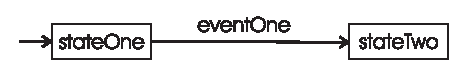
\epsfig{file=toymach.eps}
\caption{A simple state machine, called {\tt Toymachine}, which is implemented
in this section. \label{fig-toymachine}
}\end{center}
\end{figure}

\begin{codesegment}
  Transition stateOne eventOne stateTwo
  Initial stateOne
\end{codesegment}

\noindent This file specifies a State Machine module with two states and one transition. To
translate it into C++ code, we run the perl script {\tt sm-setup.pl} (for
``state machine setup'') as follows:

\medskip
\noindent{\tt > \$RHEX\_DIR/util/sm-setup.pl ToyMachine}
\medskip

\noindent This creates two generic files: {\tt ToyMachine.hh} and {\tt
ToyMachine.cc} to which we must add our own custom functionality. The first file
contains the definition of class {\tt ToyMachine} which is derived from the
virtual class {\tt StateMachine} which is derived from the virtual class {\tt
Module}. Thus a state machine is a kind of module, and therefore deals with the
Module Manager in much the same way as the modules we have already
encountered. However, the five virtual functions defined in the {\tt Module}
base class, and in particular the {\tt update()} method, are already defined in
any class that derives from {\tt StateMachine}. To give a state machine
interesting functionality, we must define the semantics of the states and
events.

First, look at {\tt ToyMachine.hh} which the perl script produced from the
{\*.dsc} file. It is as follows, except we have added a data variable called
{\tt mark} to the {\tt ToyMachine} class definition. We will use this
variable to {\em mark} the time at which the first state of the machine is
entered.

\begin{codesegment}
  #ifndef _TOYMACHINE_HH
  #define _TOYMACHINE_HH

  #include "ModuleManager.hh"
  #include "StateMachine.hh"

  class ToyMachine : public StateMachine {

    public:

      ToyMachine ( void );
      ~ToyMachine ( void );
      void init ( void );
      void activate ( void );
      void deactivate ( void );

    private:

      // events
      EventObject ( EventOne ) * eventOne;

      // states
      StateObject ( StateOne ) * stateOne;
      StateObject ( StateTwo ) * stateTwo;

      // data
      double mark;
  };

  #endif
\end{codesegment}

\noindent Note how the states and event are declared using the macros {\tt
  EventObject} and {\tt StateObject}. These macros, defined in {\tt
  Statemachine.hh}, declare new types whose scope is the {\tt ToyMachine}
  class. Thus the line

\begin{codesegment}
  EventObject ( EventOne ) * eventOne;
\end{codesegment}

\noindent does several things. First, it defines a new class {\tt EventOne}
which is derived from the virtual class {\tt Event}. Note that the scope of the
new class {\tt EventOne} does not extend beyond the {\tt ToyMachine}, thus,
other State Machines may also use the same class name without causing any
conflicts. Second, it declares this class a friend of class {\tt
ToyMachine}. And third, it sets {\tt eventOne} to be a pointer to an object of
class {\tt EventOne}. The {\tt StateObject} lines are similar.

Next, look at {\tt ToyMachine.cc}, also produced by the {\tt sm-setup.pl}
script. Here, the methods associated with the {\tt ToyMachine} class and the
state and event classes {\tt StateOne}, {\tt StateTwo} and {\tt EventOne}
and defined. This file is as follows:

\begin{codesegment}
  #include "ToyMachine.hh"

  #define OWNER ( ( ToyMachine * ) owner )

  // Events ------------------------------------------------------------
  bool ToyMachine::EventOne::check ( void ) { return false; }

  // States ------------------------------------------------------------
  void ToyMachine::StateOne::entry ( void ) {}
  void ToyMachine::StateOne::during ( void ) {}
  void ToyMachine::StateOne::exit ( void ) {}

  void ToyMachine::StateTwo::entry ( void ) {}
  void ToyMachine::StateTwo::during ( void ) {}
  void ToyMachine::StateTwo::exit ( void ) {}

  ToyMachine::ToyMachine ( void ) : StateMachine ( "toymachine" ) {

    // allocate events
    eventOne = new EventOne ( this );

    // allocate states
    stateOne = new StateOne ( this );
    stateTwo = new StateTwo ( this );

    // transitions
    Transition ( stateOne, eventOne, stateTwo );

    // the initial state
    initialize ( stateOne );

  } 

  ToyMachine::~ToyMachine ( void ) {

    if ( eventOne ) delete ( eventOne );
    if ( stateOne ) delete ( stateOne );
    if ( stateTwo ) delete ( stateTwo );

  }
 
  void ToyMachine::init ( void ) {

    StateMachine::init();

  }

  void ToyMachine::activate ( void ) {

    StateMachine::activate();

  }

  void ToyMachine::deactivate ( void ) {

    StateMachine::deactivate();

  }

\end{codesegment}

The constructor for the {\tt ToyMachine} class performs several steps. It sets
{\tt eventOne} to point to a new {\tt EventOne} object. Note that the
constructor to {\tt EventOne} requires a pointer (in this case, {\tt this}) to a
state machine class that ``owns'' the event. This will be used by the event's
method later to access the data (such as the datum {\tt mark} that we added
above) in the state machine that owns it. It then similarly sets the event
object pointers to point to new state objects. The next step sets up the
transitions in the state machine --- in this case there is only one
transition. The line

\begin{codesegment}
  // transitions
  Transition ( stateOne, eventOne, stateTwo );
\end{codesegment}

\noindent adds a {\em transition} or {\em arc} to the {\tt ToyMachine} being
constructed. The source state of the transition is {\tt stateOne}, the
destination state is {\tt stateTwo}. The event that {\em guards} the
transition from the source to the destination is {\em eventOne}. The last
step is to set up the initial state ({\tt stateOne}) of the state machine
and this is doen by the last line of the constructor.

The behavior of a {\tt ToyMachine} is as follows. When it becomes active, it
first calls the {\tt entry} method of its initial state (in this case of
{\tt stateOne}) and then continuously calls the {\tt update} method of this
state. The {\tt ToyMachine} also continuously checks the {\tt check} method
of {\tt eventOne} until it returns true. When this happens, it then calls the
{\tt exit} method of {\tt stateOne} and then then the {\tt entry} method of
{\tt stateTwo} and then continuously calls the {\tt update} function of {\tt
stateTwo}.

As it is, the script {\tt sm-setup.pl} has not put any meaning in the states
and event. It has made all the methods of {\tt stateOne} and {\tt stateTwo}
empty. And it has defined the {\tt check} method of {\tt eventOne} to always
return {\tt false}! Recall that we wanted {\tt stateOne} to be active for
one second and then for {\tt stateTwo} to be active. To arrange for this, we
first redefine the methods of {\tt stateOne} as follows:

\begin{codesegment}
  void ToyMachine::StateOne::entry ( void ) {

    OWNER->mark = MMReadTime();
    printf ( "State One Entered at Time %f\n", OWNER->mark );

  }

  void ToyMachine::StateOne::during ( void ) {}

  void ToyMachine::StateOne::exit ( void ) {
 
    printf ( "State One Exited at Time %f\n", MMReadTime() );

  }
\end{codesegment}

\noindent Now, when {\tt stateOne} is entered, it sets the datum {\tt mark}
in {\tt ToyMachine} to the current time. Note that we use the macro {\tt OWNER}
at the top of {\tt Toymachine.cc} to access the {\tt mark}. We've also added
{\tt printf} statements so that some activity may be observed when we compile
and run this machine. Now we can redefine {\tt EventOne::check}:

\begin{codesegment}
  bool ToyMachine::EventOne::check ( void ) { 

    return ( MMReadTime() >= OWNER->mark + 1.0 );

  }
\end{codesegment}

\noindent This will return true when the current time is greater than or equal to one second after
the time {\tt stateOne} was entered.

Finally, as in Section \ref{sec:together} we make a {\tt main}
function which instantiates a {\tt ToyMachine} and sets it running:

\begin{codesegment}
  #include <stdio.h>
  #include "sysutil.hh"
  #include "ModuleManager.hh"
  #include "StateMachine.hh"
  #include "ToyMachine.hh"
  #include "VirtualHW.hh"

  VirtualHW hw;

  int main( void ) {

    // declare a toy machine
    ToyMachine tm;

    MMChooseHardware( &hw );

    // Add and activate the machine
    MMAddModule( &tm, 10, 0, 10 );
    MMActivateModule( &tm );

    MMPrintModules();
    MMMainLoop();
    MMShutdown();

    return 0;
  }
\end{codesegment}

\noindent Once this code is compiled (see Section \ref{sec:worklibraries}),
it can be run to produce something like the following output:

\begin{codesegment}
  > sm 
  State One Entered at Time 2.305
  State One Exited at Time 3.305 
  >
\end{codesegment}

\noindent Note that {\tt EventOne::check()} could equally well have
corresponded to checking a remote control signal range, checking for a
pattern on a certain sensor such as touchdown of a leg, and so on. The
update functions of the two states could correspond to modes of control such
as lifting a leg to some position and so on.

\subsection{A Supervisor Machine}

In this section we construct a more complicated state machine, called {\tt
Supervisor} and shown in Figure \ref{fig-supervisor}. The basic job of the {\tt
Supervisor} machine is to activate and deactivate lower level controllers, which
may be state machines themselves, based on certain events. This particular {\tt
Supervisor} machine pays attention to remote control events reported by the {\tt
RemoteControl} module. The controllers it activates make the machine calibrate,
stand, sit and do pushups. The first three behaviors are governed by the
standard RHexLib modules {\tt CalibMachine}, {\tt StandMachine} and {\tt
SitMachine}. The last behavior is goverened by the {\tt PushupController}
constructed in Section \ref{sec-pushup}.

\begin{figure}[t]
\begin{center}
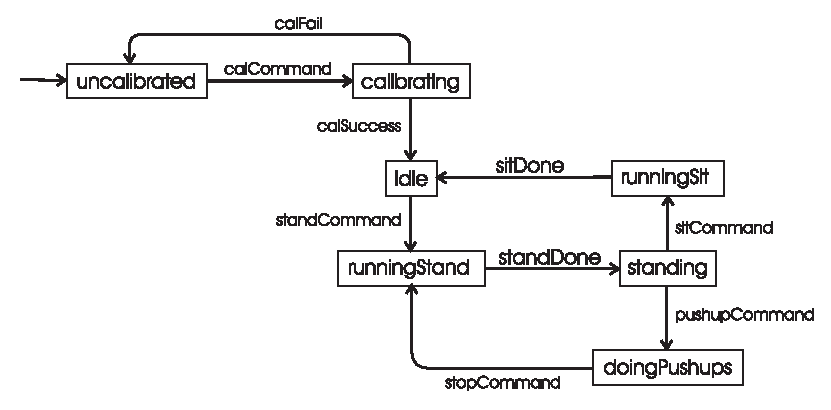
\epsfig{file=sup.eps}
\caption{A state machine, called {\tt Supervisor}, which is implemented
in this section. This machine ``supervises'' the activity of other controllers,
including other state machines. The events are either command events (which
check the remote control state) or time events. Based on the remote control
activity, the machine calibrates, stands, sits or does ``pushups''.
\label{fig-supervisor}
}\end{center}
\end{figure}

The transition table that corresponds to Figure \ref{fig-supervisor}, and which
should be saved in a file called {\tt Supervisor.dsc} is as follows:

\begin{codesegment}
  Transition uncalibrated calCommand calibrating
  Transition calibrating calFail uncalibrated
  Transition calibrating calSuccess idle
  Transition idle standCommand runningStand
  Transition runningStand standDone standing
  Transition standing sitCommand runningSit
  Transition runningSit sitDone idle
  Transition standing pushupCommand doingPushups
  Transition doingPushups stopCommand runningStand
  Initial uncalibrated
\end{codesegment}

There are seven states. {\tt uncalibrated} is the initial state, corresponding
to the situation that the robot has just been turned on. {\tt calibrating} is
the state the robot will be in while running a calibration state machine for
each leg. In the {\tt idle} state, the robot will be sitting with its motor
drives deactivated to save power. In the {\tt runningStand} state, the robot
will be running the {\tt standMachine} state machine which brings the robot to a
standing position. In {\tt standing} state, the robot will have completed the
{\tt standMachine} and will be waiting to either sit or start doing pushups. In
the state {\tt doingPushups}, the robot will be running the {\tt
pushupController} from Section \ref{sec-pushup}. Finally, in {\tt runningSit},
the robot will be running the {\tt SitMachine} controller.

There are five ``command'' events which will correspond to remote control
events. First, the {\tt calCommand::check()} method, which signals the user's intention
to calibrate the robot's legs, will be true when the left joystick is pushed
forward. The {\tt standCommand::check()} method, which signals the user's
intention to stand the robot up from idle mode, will be true when the left
joystick is pushed backward. The {\tt pushupCommand::check()} method, which
signals the user's intention to start the pushup controller from standing mode,
will be true when the left joystick is pushed forward. The {\tt
stopCommand::check()} method, which signals the user's intention to stop the
pushup controller, will be true when the left joystick is pushed backward. The
{\tt sitCommand::check()} method, which signals the user's intention to make the
robot sit when in standing mode, will be true when the left joystick is pushed
to the left.

The other events, {\tt calibSuccess}, {\tt calibFail}, {\tt standDone} and {\tt
sitDone}, correspond to the various controllers coming to completion. For
example, when the {\tt StandMachine} has finished, its {\tt isDone()} flag
returns true. Thus, {\tt standDone::check()} calls this method. As the figure
shows, while each of the controllers is running, the {\tt Supervisor} will be in
a mode that is waiting for a signal that the controller has completed, before
moving on to a state that waits for the next user input. The exception is the
{\tt doingPushups} state, which is terminated upon a remote control action from
the user.

\subsubsection{Coding the Supervisor}

We will see that there are very few things to be done to code up this seemingly
complex state machine. First, we use {\tt sm-setup.pl} to create skeleton header
and code files from the {\tt Supervisor.dsc} file. This creates 90\% of the code
for the {\tt Supervisor} machine.

The header, {\tt Supervisor.hh}, is practially finished. We just need to include
certain header files from RHexLib which define the other machines to be used and
add variables to the Supervisor class to point to the modules it will need. We
also suppose that {\tt PushupController.hh} has been created and placed in the
same directory as the supervisor code. The resulting header file is as follows:

\begin{codesegment}
#ifndef _SUPERVISOR_HH
#define _SUPERVISOR_HH

#include "ModuleManager.hh"
#include "StateMachine.hh"

// The next six includes have been added to the basic
// file produced by sm-setup.pl
#include "StdModules.hh"
#include "StandMachine.hh"
#include "SitMachine.hh"
#include "CalibMachine.hh"
#include "RemoteControl.hh"
#include "PushupController.hh"

class Supervisor : public StateMachine {

  public:

    Supervisor ( void );
    ~Supervisor ( void );
    void init ( void );
    void activate ( void );
    void deactivate ( void );

  private:

    // events
    EventObject ( CalCommand ) * calCommand;
    EventObject ( CalFail ) * calFail;
    EventObject ( CalSuccess ) * calSuccess;
    EventObject ( StandCommand ) * standCommand;
    EventObject ( StandDone ) * standDone;
    EventObject ( SitCommand ) * sitCommand;
    EventObject ( SitDone ) * sitDone;
    EventObject ( PushupCommand ) * pushupCommand;
    EventObject ( StopCommand ) * stopCommand;

    // states
    StateObject ( Uncalibrated ) * uncalibrated;
    StateObject ( Calibrating ) * calibrating;
    StateObject ( Idle ) * idle;
    StateObject ( RunningStand ) * runningStand;
    StateObject ( Standing ) * standing;
    StateObject ( RunningSit ) * runningSit;
    StateObject ( DoingPushups ) * doingPushups;

    // These six pointers have been added to the basic file produced
    // by sm-setup.pl. They will point to other modules used by the Supervisor
    PushupController * puControl;
    StandMachine     * standMach;
    SitMachine       * sitMach;
    CalibMachine     * cm[6];
    Hardware         * hw;
    RemoteControl    * rc;

};

#endif
\end{codesegment}

The next step is top modify the code file, {\tt Supervisor.cc}, produced by
{\tt sm-setup.pl}. We will do this in several steps:
\begin{enumerate}
\item Modify {\tt Supervisor::activate()} to search for the required modules
(for standing, sitting, etc.) and set up the module pointers that we added to
{\tt Supervisor.hh}.
\item Modify {\tt Supervisor::activate()} and {\tt Supervisor::deactivate()} to
grab and release the remote control module.
\item Modify the event {\tt check()} methods to check for remote control events
and controller {\tt isDone()} events.
\item Modify the state {\tt entry()}, {\tt during()} and {\tt exit()} methods
(not all of them) so that they activate and deactivate the various modules
responsible for calibrating, standing, sitting and doing pushups.
\end{enumerate}

\noindent First we modify the {\tt init()} method to search for the required modules. We
also setup the {\tt hw} pointer to point to the currently instantiated hardware
object. This is needed to enable and turn off the motor drives. The {\tt init()}
method is then:

\begin{codesegment}
void Supervisor::init ( void ) {

  int i;

  // this is where to search for the needed modules and set up pointers to them

  if ( ( standMach = ( StandMachine * ) 
         MMFindModule( STANDMACHINE_NAME, 0 )) == NULL)
     MMFatalError ( "Supervisor::init", "Cannot find Stand Machine" );
  
  if ( ( sitMach = ( SitMachine * ) 
         MMFindModule( SITMACHINE_NAME, 0 )) == NULL)
     MMFatalError ( "Supervisor::init", "Cannot find Sit Machine" );
  
  if ( ( rc = ( RemoteControl * ) 
         MMFindModule( REMOTECONTROL_NAME, 0 )) == NULL)
     MMFatalError ( "Supervisor::init", "Cannot find Remote Control" );

  if ( ( puControl = ( PushupController * ) 
         MMFindModule( "pushupcontroller", 0 )) == NULL)
     MMFatalError ( "Supervisor::init", "Cannot find Push Up Controller" );

  for ( i = 0; i < 6; i++ )
    if ( ( cm[ i ] = ( CalibMachine * ) 
           MMFindModule( CALIBMACHINE_NAME, i )) == NULL)
      MMFatalError ( "Supervisor::init", "Cannot find Calibration Machine" );

  hw = MMGetHardware();

  StateMachine::init();

}
\end{codesegment}

\noindent Next, we modify the {\tt activate()} and {\tt deactivate()} methods so
that they grab, configure and release the remote control module. The arguments
to {\tt rc->configure} are the delays of the right and left joystick inputs. A
deley of 0.005$s$, for example, means that the value has to be stable for 0.005
seconds before it is reported. The {\tt rc->setThreshold} method sets the value
above which the joystick is considered to be pushed in a particular
direction. In the {\tt deactivate()} method, we also check to see if any of the
modules that the {\tt Supervisor()} uses are active, and if they are, we
deactivate them.

\begin{codesegment}
void Supervisor::activate ( void ) {

  // Configure the RC sticks
  rc->configure ( 0.005, 0.3 );
  rc->setThreshold ( 0.5 );

  // Grab and activate the remote control interface
  MMGrabModule( rc, this );

}

void Supervisor::deactivate ( void ) {

  // Release the previously grabbed modules
  MMReleaseModule( rc, this );

  if ( standMach->getState() == MODULE_ACTIVE ) MMReleaseModule ( standMach, this );
  if ( sitMach->getState() == MODULE_ACTIVE ) MMReleaseModule ( sitMach, this );
  if ( puControl->getState() == MODULE_ACTIVE ) MMReleaseModule ( puControl, this );

  for ( i=0; i<6; i++ )
    if ( cm[i]->getState() == MODULE_ACTIVE ) MMReleaseModule ( cm[i], this );

  StateMachine::deactivate();

}
\end{codesegment}

\subsubsection{The Event {\tt check()} Methods}

Next, we add meaning to the event {\tt check()} methods. We start with {\tt
calibCommand}. This amounts to checking the value returned by the {\tt
rc->leftSick} and {\tt rc->rightStick} methods. The values returned by these
methods correspond to the cardinal map directions (north, west, northwest, etc.)
Thus, the {\tt calibCommand::check()} method below returns true if the left
joystick is pushed directly forward.

\begin{codesegment}
bool Supervisor::CalCommand::check ( void ) { 

  // Left RC stick pushed forward
 return bool ( OWNER->rc->leftStick() == RemoteControl::NORTH );

}
\end{codesegment}

\noindent The next two events check for either the sucessful completion of all the
calibration machines (one for each leg) or the unsucessful completion of at
least one of them. {\tt CalibMachine::getStatus} returns {\tt
CalibMachine::FAILURE} in the case that calibration failed, {\tt
CalibMachine::CALIBRATING} if calibration is still underway and {\tt
CalibMachine::SUCCESS} if calibration suceeded.

\begin{codesegment}
bool Supervisor::CalFail::check ( void ) {

  int i;

  // return true if any motor reports failure
  for ( i = 0; i < 6; i++ )
    if ( OWNER->cm[i]->getStatus() == CalibMachine::CALIBRATING ) return false;
  for ( i = 0; i < 6; i++ )
    if ( OWNER->cm[i]->getStatus() == CalibMachine::FAILURE ) return true;
  
  return false;

}

bool Supervisor::CalSuccess::check ( void ) {

  // return true if all motors report success
  int i;

  for ( i = 0; i < 6; i++ )
    if ( OWNER->cm[i]->getStatus() != CalibMachine::SUCCESS ) return false;
  
  return true;

}
\end{codesegment}

\noindent The stand command is issued by pushing the left joystick directly backward.

\begin{codesegment}
bool Supervisor::StandCommand::check ( void ) { 

  // Left RC stick pushed back
  return bool ( OWNER->rc->leftStick() == RemoteControl::SOUTH );

}
\end{codesegment}

\noindent Via the public interface to {\tt StandMachine}, other modules can
perceive two states. Either the machine is in the midst of standing, in which
case {\tt StandMachine::isDone()} returns {\tt false} or the machine is
completed its task and is holding steady, and {\tt isDone()} returns {\tt true}.

\begin{codesegment}
bool Supervisor::StandDone::check ( void ) { 

  return OWNER->standMach->isDone();

}
\end{codesegment}

\noindent To sit, push the left joystick directly to the left.

\begin{codesegment}
bool Supervisor::SitCommand::check ( void ) {

  // Left RC stick pushed left
  return bool ( OWNER->rc->leftStick() == RemoteControl::WEST );

}
\end{codesegment}

\noindent The {\tt SitMachine} interface is similar to the {\tt StandMachine} interface.

\begin{codesegment}
bool Supervisor::SitDone::check ( void ) {

  return OWNER->sitMach->isDone();

}
\end{codesegment}

\noindent To start doing pushups, push the joystick directly forward while in standing mode.

\begin{codesegment}
bool Supervisor::PushupCommand::check ( void ) {

  // Left RC stick pushed forward
  return bool ( OWNER->rc->leftStick() == RemoteControl::NORTH );

}
\end{codesegment}

\noindent To stop doing pushups, push the left joystick directly backward.

\begin{codesegment}
bool Supervisor::StopCommand::check ( void ) {

  // Left RC stick pushed back
  return bool ( OWNER->rc->leftStick() == RemoteControl::SOUTH );

}
\end{codesegment}

\subsubsection{The State Methods}

The next and final step is to modify the state methods. Note that we do not
modify them all as they are not all needed. For example, none of the {\tt
during()} methods are changed at all as will often be the case in supervisor
state machines. To see how the {\tt during()} methods are used, see the code of,
for example, {\tt StandMachine}. Here, only {\tt some} of the {\tt entry()} and
{\tt exit()} methods are actually required. Mostly what they do is activate and
deactivate other modules. Activation of a module is done with the {\tt
MMGrabModule} function. Deactivate is done with the {\tt MMReleaseModule()}
function.

There are six caibration machines to be activated upon entry into the {\tt
calibrating} state as follows. This method also sets the calibration method of
each machine to {\tt GROUND} which makes the robot's legs spin until the meet
with some resistance (persumably the ground).

\begin{codesegment}
void Supervisor::Calibrating::entry ( void ) {

  int i;

  for ( i = 0; i < 6; i++ ) {

    OWNER->cm[i]->setMode( CalibMachine::GROUND );
    MMGrabModule ( OWNER->cm[i], owner );

  }
}
\end{codesegment}

\noindent Upon completion of the {\tt calibrating} state, when either {\tt calibSucess}
or {\tt calibFail} become active, we release the calibration machines, thereby
deactivating them.

\begin{codesegment}
void Supervisor::Calibrating::exit ( void ) {

  int i;

  for ( i = 0; i < 6; i++ )
    MMReleaseModule ( OWNER->cm[i], owner );
}
\end{codesegment}

\noindent Successful calibration leaves the robot calibrated with the motor
drives off. Thus, to start standing, we need to enable the motor drives and
then grab the stand machine.

\begin{codesegment}
void Supervisor::RunningStand::entry ( void ) {

  int i;

  for ( i = 0; i < 6; i++ )  // enable motor drives
    OWNER->hw->driveEnable( i, true );
  
  MMGrabModule ( OWNER->standMach, owner );
}
\end{codesegment}

\noindent We leave the standing machine running during the {\tt standing}
state though it is in the standing position. This is because the {\tt
StandMachine} holds the robot in the upright position after it is done. We
release (and deactivate) the standing machine only when leaving the {\tt
standing} state on our way either to sitting or doing pushups.

\begin{codesegment}
void Supervisor::Standing::exit ( void ) {

  MMReleaseModule ( OWNER->standMach, owner );

}
\end{codesegment}

\noindent To start sitting, we grab the sit machine (don't let anyone just anyone grab
your sit machine!).

\begin{codesegment}
void Supervisor::RunningSit::entry ( void ) {  

  MMGrabModule ( OWNER->sitMach, owner );

}
\end{codesegment}

\noindent When the {\tt SitMachine} is done, we release it and also disable
the motor drives to save power.

\begin{codesegment}
void Supervisor::RunningSit::exit ( void ) {

  int i;

  for ( i = 0; i < 6; i++ )  // disable motor drives
    OWNER->hw->driveEnable( i, false );

  MMReleaseModule ( OWNER->sitMach, owner );
}
\end{codesegment}

\noindent Finally, it is easy to incoorporate the pushup controller, we just grab and
release it as needed:

\begin{codesegment}
void Supervisor::DoingPushups::entry ( void ) {

  MMGrabModule ( OWNER->puControl, owner );

}

void Supervisor::DoingPushups::exit ( void ) {

  MMReleaseModule ( OWNER->puControl, owner );

}
\end{codesegment}

\subsubsection{A {\tt main()} File}

One more piece is required to get the {\tt Supervisor} runnning. We need a main
file. The following will do.

\begin{codesegment}
#include <stdio.h>
#ifdef _QNX4_
#include <sys/sched.h>
#include <unistd.h>
#endif
#include "sysutil.hh"
#include "ModuleManager.hh"
#include "StdModules.hh"
#include "StateMachine.hh"
#include "Supervisor.hh"
#include "RemoteControl.hh"
#include "PushupController.hh"
#include "MichiganHW.hh"

MichiganHW hw;

class UserModule : public Module {

  public:

    UserModule ( void ) : Module( "userinput", 0, false, false ) { };

    void  init ( void ) {}
    void  uninit ( void ) {}
    void  activate ( void ) {}
    void  deactivate ( void ) {}
    void  update ( void ) {

      int i;

      if ( kbhit() ) {

        // Diable all motor drives
        for ( i = 0 ; i < 6 ; i++) 
          hw.driveEnable ( i, false );

        MMShutdown();
        MMPowerOff( );

      }
    }
} umod;

int main ( void ) {

#ifdef _QNX4_
  setprio( getpid(), 23 );
#endif

  MMReadConfigFile( "rhex_michigan.rc" );

  // Read the application dependent configuration file
  MMReadConfigFile( "sup.rc" );

  MMChooseHardware ( & hw );

  Supervisor supervisor;
  PushupController puc;

  // Create and add all the standard modules
  RHexAddStdModules();

  // Add the user module, pushup controller and supervisor
  MMAddModule ( &umod, 1, 0, USER_CONTROLERS );
  MMAddModule ( &puc, 1, 0, USER_CONTROLLERS );
  MMAddModule ( &supervisor, 1, 0, USER_CONTROLLERS );

  // Activate the supervisor modules
  MMActivateModule ( &supervisor );

  MMMainLoop();
  MMShutdown();
  return 0;

}
\end{codesegment}

The machines for calibration, standing and sitting as well as the
remote control module are all added to the Module Manager by the command {\tt
RHexAddStdModules()}. Only the {\tt Supervisor} and the {\tt PushupController}
are added in {\tt main()}. Also, only the {\tt Supervisor} module is activated
in {\tt main()}. It takes care of activating everything else it needs. We have
also added a simple module, called {\tt UserModule}, which allows the user to
stop the program by pressing any key.

Note, we have
chosen to configure this program to use the {\tt Michigan.hh} hardware library
and the {\tt rhex\_michigan.rc} file.

\section{Hardware Components}

This section gives a tutorial on how to deal with Hardware interfaces in
RHexLib. The following sections briefly explain and give examples on how to
accomplish increasingly complex tasks related to RHexLib's low level
hardware interface.

Section \ref{sec:using_hardware} outlines how to use one of the existing
Hardware components. Section \ref{sec:unsupported_hardware} explains how to
access a piece of hardware currently unsupported by the interface. Section
\ref{sec:adding_hardware} presents how to augment the Hardware class
interface with a new type of component, which is general and useful enough
to be implemented by all versions of the hardware. Finally, Section
\ref{sec:new_hardware_class} outlines how to create a completely new
hardware library, conforming to the interface of the Hardware class whose
implementation is different from the existing hardware libraries.

\subsection{Using the Hardware Class Interface}
\label{sec:using_hardware}

RHexLib solves the issue of being able to use the same higher level control
code with different versions of the underlying low level hardware (such as
encoders, analog IO, digital IO etc.) by the use of {\em hardware
libraries}, instantiating specific implementations of the {\tt Hardware}
class and the associated component classes. The abstract base templates for
these classes are defined in {\tt Hardware.hh} and their class interfaces
are explained in detail in Chapter \ref{sec:hardware_interface}.

As a consequence, the first thing that any RHexLib program does is to create
an instance of the desired hardware class, which are always inherited from
the abstract base class {\tt Hardware}. Currently, RHexLib distribution
defines {\tt MichiganHW}, {\tt McGillHW}, {\tt SimSectHW} and {\tt
  VirtualHW}, supporting the Michigan RHex, McGill RHex, SimSect simulation
interface and a simple simulator for free running motors,
respectively. Usually, the hardware object is created as a global object
(whose constructor is called before main() is executed) in one of the source
files.

\begin{codesegment}
#include "SimSectHW.hh"
SimSectHW hw;
\end{codesegment}

The next thing that needs to be done is to inform the module manager about
the newly created hardware object, making it possible for all modules and
components in the system to get their hands on this object for low level
hardware access. This is accomplished with the {\tt MMChooseHardware()}
function, which calls the appropriate initialization methods of the hardware
object. Usually, this function is called {\em after} loading the
configuration symbol table because often, the initialization of the hardware
accesses the configuration symbols.

\begin{codesegment}
int main( int argc, char **argv ) {

  MMReadConfigFile( "rhex_standard.rc" );
  MMChooseHardware( &hw );

  // the rest of main() code goes here...

  MMMainLoop(); // Invoke the main module manager loop
}
\end{codesegment}

Once these steps are completed, then all the modules and components in the
system can access low level hardware functionality through this
object. However, due to the data abstraction principles, module
implementations must {\em never} rely on the presence of a global module
object. Different programs might instantiate this object with different
names, or maybe even not as a global variable. Therefore, the {\tt
  MMGetHardware()} function is provided to acquire a pointer to the current
hardware object through the module manager's central database. Usually,
modules acquire this pointer in their {\tt init()} methods and store it
locally.

\begin{codesegment}
void DummyModule::init( void ) {

  local_hw_ptr = MMGetHardware();

  // Rest of the init() code...
}
\end{codesegment}

The Hardware class itself provides a few methods to access some general
hardware facilities such as reading the clock, enabling/disabling motor
drives ({\em *TODO*: This should probably be part of DCMotorHW instead of
  the Hardware class}) etc. The details of these methdos are explained in
Section \ref{sec:hardware_class}.

In contrast, the functionality related to individual hardware components are
accessed through component class interfaces. The Hardware class holds
pointers to instances of these interfaces, through which modules can get
access to component specific functionality. For example, 

\begin{codesegment}
  uint16 count = local_hw_ptr->encoders->read( 3 );
\end{codesegment}

\noindent would read the 16 bit encoder count for the third axis. Current,
the Hardware class has pointers to a few standard component types, all of
which are explained in detail in Chapter \ref{sec:hardware_interface}.

\begin{classdef}
class Hardware {
public:

  // Some other stuff...

  EncoderHW   * encoders;
  AnalogHW    * analogIO;
  DigitalHW   * digitalIO;
  TimerHW     * timers;
  AccelHW     * accels;
  GyroHW      * gyros;
  PowerHW     * power;
  SwitchHW    * switches;
  DialHW      * dials;
  DCMotorHW   * dcmotors;
};
\end{classdef}

One {\em very important} feature to note is that, these fields are
initialized to {\tt NULL} if the particular hardware implementation does not
support the corresponding component. As a consequence, it is {\tt always} a
good idea for a module to check the presence of a desired hardware component
in the init function, and exit with a fatal error if it does not exist.

\begin{codesegment}
void DummyModule::init( void ) {

  local_hw_ptr = MMGetHardware();

  if ( local_hw_ptr->encoders == NULL )
    MMFatalError( "DummyModule::init", 
                  "Encoder Hardware component not supported!" );

  if ( local_hw_ptr->analogIO == NULL )
    MMFatalError( "DummyModule::init", 
                  "Analog I/O Hardware component not supported!" );

  // Rest of the init() code...
}
\end{codesegment}

Note that this kind of error checking does not introduce any runtime
inefficiency because it is done only once when the module is added through
{\tt MMAddModule()}.

\subsection{Accessing an Unsupported Piece of Hardware}
\label{sec:unsupported_hardware}

Suppose you wanted to quickly add a sensor or actuator, which is not
included in the set of standard components of Chapter
\ref{sec:hardware_interface}. This section explains how this can easily be
done.

Obviously, augmenting the Hardware interface by adding another component
seems to be the natural solution. However, this is relatively time consuming
and involves modifying the core library distribution, which should be
avoided for prototyping purposes. Section \ref{sec:adding_hardware} explains
how this can be done in cases where the component in question is {\em
extremely} useful and you believe that it should definitely be part of the
standard set of components. However, even then, testing the component and
its interface through the methods described in this section is the best
first solution.

In this context, there are two scenarios, which call for two different
solutions. If the sensor in question only requires a few I/O instructions
(possibly using the existing hardware components such as the analog I/O) and
no significant processing, then you need to write a simple non-module class
to encapsulate the interface. For example, for a range sensor which is
connected to the analog inputs and only requiring a simple affine mapping to
obtain the range data, you could create a class {\tt RangeSensor}.

\begin{classdef}
class RangeSensor {
  public :

    RangeSensor( uint analog_channel ) { 

      local_hw_ptr = MMGetHardware();

      if ( ( local_analogio_ptr = local_hw_ptr->analogIO ) == NULL )
        MMFatalError( "RangeSensor::RangeSensor",
                      "Analog I/O hardware component does not exist" );
      channel = analog_channel; 
    };
  
    float read( void ) { 
      return analog_to_range( local_analogio_ptr->read( channel ) );
    };

  private:

    float analog_to_range( float analog_value );

    Hardware *local_hw_ptr;
    AnalogIO *local_analogio_ptr;
    uint     channel;
};
\end{classdef}

From this point on, anybody who wants to use the range sensor would create
an instance of this class and access the range value through {\tt
  RangeSensor::read()} method. Note that the {\tt analog\_to\_range()} method
is where the conversion to the range value is performed. If you think this
much code is unnecessary and want to do it the dirty way, you could simply
write a global {\tt AnalogToRange()} function and use it on a direct reading
from the analog inputs.

There may be cases, however, where the processing required to perform the
conversion is too long and should be performed only once per cycle for
efficiency purposes. It might also be the case that the sensor's output is
based on a time history of a data stream, such as a filtered sensor. In
those cases, such a simple class interface will not be sufficient and you
will need to create a {\em Module}.

Defining such a module will make it possible to do processing only once per
cycle in the module's update function, and provide access to the hardware
component's functionality through local interface methods. In the rest of
this section, we will work out an example of such a module, implementing a
simple filtered version of the above range sensor.

\begin{classdef}
class RangeSensorModule : public Module {
  public:

    RangeSensorModule::RangeSensorModule( uint analog_channel );

    float read( void ) { return range; };

    void init( void ) { };
    void uninit( void ) { };
    void activate( void );
    void deactivate( void ) { };
    void update( void );

  private:

    float analog_to_range( float analog_value );

    float range;
};
\end{classdef}

The module's update function will handle reading the analog input, filtering
and storing the latest filtered value in the private member {\tt
  range}. Also, we need to implement the {\tt activate()} function to reset
the internal filter state.

The module constructor is very similar to the RangeSensor class. One small
difference is that, we use the module {\em index} to store the analog
channel number in this case. This is accomplished by creating the base
Module class with name {\tt "rangesensor"}, the index corresponding to the
analog channel as a multi-user, non-polling module. A consequence of this is
that, you will be able to create only one {\tt RangeSensorModule} module for
a particular analog input channel because two modules with the same name and
index cannot coexist in the module manager.

\begin{codesegment}
RangeSensorModule::RangeSensorModule( uint analog_channel )
  : Module( "rangesensor", analog_channel, false, false ) {

  local_hw_ptr = MMGetHardware();

  if ( ( local_analogio_ptr = local_hw_ptr->analogIO ) == NULL )
    MMFatalError( "RangeSensorModule::RangeSensorModule",
                  "Analog I/O hardware component does not exist" );
};
\end{codesegment}

The activate function is very simple and simply resets the range value to
its initial value. Note the use of the {\tt getIndex()} method from the base
Module class to obtain the analog channel number.

\begin{codesegment}
void RangeSensorModule::activate( void ) {

  range = analog_to_range( local_analogio_ptr->getIndex() );
};
\end{codesegment}

Finally, the bulk of the work is done in the update method. We use an
exponantial filter, which computes the range as a weighted sum of the
previous range value and the current raw range reading from the analog
channel. We used hard-coded weight values, although these values could
easily be configurable through some module methods or configuration
variables.

\begin{codesegment}
void RangeSensorModule::update( void ) {

  float unfiltered_range;

  unfiltered_range = analog_to_range( local_analogio_ptr->getIndex() );

  range = 0.9 * range + 0.1 * unfiltered_range;
};
\end{codesegment}

This implementation is very efficient because it only reads the analog input
and filters the signal once per cycle. Even if the range value is read 100
times per cycle, it is computed only once.

\subsection{Adding a Component to the Hardware Class Interface}
\label{sec:adding_hardware}

So, if you are reading this section, it means that you have decided the
hardware component that you want to add is generic enough that it deserves
to be in the standard set of hardware components. Even though the
modifications necessary to accomplish this are minimal and will have no
effect on the rest of the system, there are a couple of issues to be
considered before you plunge ahead.

\begin{itemize}
\item{In RHexLib, the hardware layer is designed to capture the {\em
minimal} functionality regarding low level hardware access, which is
platform dependent. It is {\em extremely} important to limit the scope of
the component that you want to add to the smallest possible set of
functionality which you think will be different for different versions of
the robot or the simulation. In most of the cases, it should simply deal
with raw data acquisition and possibly some basic unit
conversions. Everything else should be implemented separately, either as
modules or classes. This makes it possible to reuse all the hardware
independent code for all hardware versions.

For example, in defining the {\tt GyroHW} class, we did not put the
procedures for integrating the angular velocities or estimating body state
below the hardware layer. Instead, the only hardware dependent
functionality, which is the acquision of the angular rate information from
the physical (or simulated) hardware is implemented through {\tt GyroHW}
interface. The rest of the functionality is independent of which hardware is
used, and can be implemented in the form of commonly usable modules.}
\item{Everybody who will use the library in the future will be forced to use
the new component interface that you are about to design. Consequently, it
is extremely important that all current developers of the library (at least
the core set of people) should have a chance to comment on the interface you
propose. Before starting any implementation, you should collect these
opinions.}
\end{itemize}

Having considered these issues, the first step is to define the interface of
the hardware component. As an example, we will design an LCD text/graphics
display interface component, {\tt LCDisplayHW}.

Following the above guidelines, we would like this interface to be as
general as possible, while limiting its scope to only hardware dependent
functionality. We would like the interface to support both text and graphics
modes in black and white, as well as a way to figure out which modes are
possible in a particular instantiation. While in text mode, the basic
operation is to put an ASCII character on a given coordinate. 

In contrast, the graphics mode requires the ability to modify individual
pixels, as well as pasting a rectangular graphics object to a given location
on the display. Other methods such as drawing rectangles, lines circles
etc. would have been possible, but we leave those out for simplicity.

The following class definition outlines the interface we propose. This
definition should go in {\tt Hardware.hh}, before the {\tt Hardware} class
definition. 

\begin{classdef}
class LCDisplayHW {
  public:
    virtual ~LCDisplayHW( ) { };

    typedef enum { TEXT_MODE = 0x01, GRAPHICS_MODE = 0x02 } DisplayMode;

    virtual bool        setMode ( DisplayMode newMode ) = 0;
    virtual DisplayMode getMode ( void ) = 0;

    virtual void clearDisplay ( void ) = 0;
    virtual void getDisplaySize ( int *width, int *height ) = 0;

    virtual bool writeChar ( uint x, uint y, char c ) = 0;
    virtual char readChar ( uint x, uint y ) = 0;

    virtual bool getPixel ( uint x, uint y ) = 0;
    virtual bool setPixel ( uint x, uint y, bool val ) = 0;
    virtual bool pasteBitmap ( uint x, uint y, 
                               uint width, uint height, char *bitmap ) = 0;
};
\end{classdef}

Note that all the methods are defined as pure virtual functions because the
real work will be done in classes inherited from {\tt LCDisplayHW} in
specific hardware libraries. We will not give the details of what each of
these methods are supposed to do as it is pretty obvious from their names
and arguments. This collection of methods covers quite a large number of
display types and is an appropriate start for the desired functionality. We
kept this example simple for documentation purposes, but the interface
certainly could be augmented to handle more complicated features.

Having decided on the component interface and defined the component class
{\tt LCDisplayHW}, the next step is to change the {\tt Hardware} class to
support the new component. Two modifications are needed: Adding a pointer to
an instance of the new component to the Hardware class public members, and
changing the Hardware class constructor to initialize this pointer to {\tt
NULL}.

\begin{classdef}
class Hardware {
public:

  Hardware( void ) { 
    lcdisplay = NULL;      // <<<<< New addition.
    encoders = NULL; 
    analogIO = NULL; 

    // ( Some other NULL assignments which were already there... )

  };

  // ( Some unrelated method declarations ... )

  LCDisplayHW * lcdisplay; // <<<<< New addition.
  EncoderHW   * encoders;

  // (Some other pointers which were already there ... )

};
\end{classdef}

These are all the modifications needed to the core library. The remaining
steps involve the actual implementation in a specific hardware library. Note
that initially, you will only need to change the hardware library that you
will immediately be working with. {\em You do not need to change any other
library as this point}. The member variable {\tt lcdisplay} will by default
be {\tt NULL}, which means that this component will simply be unsupported by
the other existing libraries. Any module that follows the guidelines of
Section \ref{sec:using_hardware} will notice this in their {\tt init()}
function and give a fatal error in the presence of a library which does not
support this component.

The final steps hence involve augmenting your current hardware library with
a specific implementation of this component. For this example, we will
change {\tt MichigahHW} class.

First, we define a new class, inherited from {\tt LCDisplayHW}, where all
the real work will be done. The following code would go into {\tt
  UMichHW.hh} in {\tt hardware/UofM/UMichLCD.hh} and is internal to the
hardware library and will not be visible to any user of RHexLib.

\begin{classdef}
class UMichLCD : LCDisplayHW {
  public:
    UMichLCD( void )
    ~UMichLCD();

    bool        setMode ( DisplayMode newMode );
    DisplayMode getMode ( void );

    void clearDisplay ( void );
    void getDisplaySize ( int *width, int *height );

    bool writeChar ( uint x, uint y, char c );
    char readChar ( uint x, uint y );

    bool getPixel ( uint x, uint y );
    bool setPixel ( uint x, uint y, bool val );
    bool pasteBitmap ( uint x, uint y, 
                       uint width, uint height, char *bitmap );
};
\end{classdef}

Note that all the pure virtual functions of the base class are implemented
by this new class. We will not give the code for these methods, but remember
that these methods will be where all the hardware access, buffering, low
level I/O etc. are done. Usually, it a good idea to create separate files
for the implementations of each hardware component.

Now to the final step. The {\tt MichiganHW} class is inherited from the base
{\tt Hardware} class and is responsible from filling in the component
pointers for the pieces of hardware that it supports. As a consequence, we
now need to go in {\tt hardware/UofM/MichiganHW.cc} and change the method
{\tt MichiganHW::initialize()} to create an instance of {\tt UMichLCD} and
initialize the corresponding component pointer.

\begin{codesegment}
void MichiganHW::initialize( void ) {

  // ( Some unrelated initialization code ... )

  lcdisplay = new UMichLCD;        // <<<<< New addition.
  encoders = new MEncoder;
  // ( Initialization of other pointers ... )

  // ( Some other unrelated initialization code ... )
}
\end{codesegment}

Similarly, you will need to change the method {\tt MichiganHW::cleanup()} to
delete the created component object.

\begin{codesegment}
void MichiganHW::cleanup( void ) {

  // ( Some unrelated cleanup code ... )

  if ( lcdisplay != NULL ) delete lcdisplay;        // <<<<< New addition.
  if ( encoders != NULL ) delete encoders;
  // ( Cleanup of other pointers ... )

  // ( Some other unrelated cleanup code ... )
}
\end{codesegment}

This completes the necessary changes to access your new LCD through its
uniform class interface. Maintainers of other hardware libraries can augment
their own implementations to support their particular LCD hardware, at which
point they will be able to use all of you higher level modules accessing the
LCD component. 

\subsection{Creating a New Hardware Class}
\label{sec:new_hardware_class}

When a new major hardware revision is made, or when RHexLib is being ported
to a completely different platform, a new hardware library will need to be
created. Even though all of the principles and methods explained in previous
sections will still apply, creating a new hardware library is somewhat more
complicated and involves a lot more coding. Before proceeding, please read
Chapter \ref{sec:hardware_interface} for the details of the Hardware class
and the supported hardware components.

The first step is to decide on a name for the new Hardware class to be
created. The name should be sufficiently descriptive, keeping in mind that
there may be later hardware libraries with similar names. Even though it is
possible to use an existing Hardware class name, keeping different
implementations in different directories and libraries, it is better to have
different class names as it will avoid later confusion.

In this section, we will present an example hardware class, {\tt ExampleHW},
together with how to implement the standard set of components and add the
resulting library to the distribution.

The RHexLib core distribution includes a directory, {\tt hardware}, which
contains individual directories for each of the supported hardware
libraries. Normally, the newly created library and the associated files
would go into a separate directory under {\tt hardware}. However, for
testing and debugging purposes, it is best to start in a local directory of
your own. Let's name it {\tt example} for the time being.\\

\noindent{\tt
\# cd \~{}/RHex/UlucDevel \\
\# mkdir hardware \\
\# mkdir hardware/example \\
\# cd hardware/example \\
}

The next step is to create the Makefile which will generate the library. You
can copy one from {\tt tools/Makefile.libsample} and change the lines {\tt
  LIBRARY}, {\tt SOURCES} and {\tt AUXFLAGS} as necessary. For our example,
we will name the library {\tt libexamplehw.a}. The {\tt SOURCES} line will
be completed as we add more sources. Finally, {\tt AUXFLAGS} should contain
any additional compilation flags, such as include search paths and library
search paths.

At this point, we are ready to create the main hardware header file, which
will be the only visible component of the hardware library to the users of
RHexLib. When the new library becomes part of RHexLib core distribution,
this header file will go into the {\tt include} directory, from where
anybody can include it. For now, create the file {\tt ExampleHW.hh} in your
local directory with the appropriate license headers and the following class
definition.

\begin{classdef}
#include "Hardware.hh"

class ExampleHW : public Hardware {

public:
  ExampleHW( void );
  ~ExampleHW( );

  void initialize( void );
  void cleanup( void );

  CLOCK readClock( void );
  CLOCK readUClock( void );

  void driveEnable( uint index, bool enable );
};
\end{classdef}

The implementations of these methods would go into {\tt ExampleHW.cc}. We
will describe what needs to be done in each of these e in later paragraphs.

The next step is to define implementations for each of the standard
components supported by the Hardware interface. For this purpose, you need
to create a header file {\tt ExComponents.hh}, where you define classes
derived from each of the components your hardware library will support. Note
that you do not need to support all the components, but be aware that what
you leave unsupported will prevent controllers using those components from
functioning. This header file will be local to the library and will not be
visible by the users of the library.

\begin{classdef}
#include "Hardware.hh"

class ExEncoder : public EncoderHW {
public:
  ExEncoder( void );
  ~ExEncoder( );

  void   enable( uint index );
  void   disable( uint index );
  uint16 read( uint index );
  void   reset( uint index );
};

class ExAnalog : public AnalogHW {
public:
  ExAnalog( void );
  ~ExAnalog( );

  float read( uint index );
  void  write( uint index, float value );
  void  outputRange( uint index, float *min, float *max );
  float readOutput( uint index ) { return output[index]; };
};

// Followed by definitions of other components.
\end{classdef}

You can add other private or public methods and members to these
classes. However, keep in mind that they will NOT be part of the standard
Hardware class interface and they should only be used locally by the files
in the library that we are about to create.

The next stage is where the bulk of the work is done. It involves
implementing the methods of each of these components, in a way that conforms
with the specifications of Chapter \ref{sec:hardware_interface}. The
implementation is completely up to you, although you can look at the
existing hardware libraries as examples.

Usually, there are pieces of hardware, such as PC104 cards etc. which have
functionality corresponding to more than one of these hardware
components. In that case, it is a very good idea to create a separate class
interface to access that piece of hardware, which is then used by these
component interfaces to implement specific functionality. Examples of such
classes can be found in the {\tt hardware/common} directory. The {\tt
dm6814} and {\tt mpc550} classes are designed precisely for that purpose.

At this point, we will need to go back and explain what the {\tt initialize}
and {\tt cleanup} methods of the {\tt Hardware} class are for. When a
RHexLib program calls {\tt MMChooseHardware()}, the {\tt initialize()}
method of the hardware class is called. In this method, you must do all
proper initialization of the hardware, as well as making sure that only one
instance of the same hardware object is created. The following list
summarizes what needs to be done in this method.

\begin{itemize}
\item{Check whether another instance of this hardware object was created
before. If so, give an error because only one hardware object should exist
in the system at once. You can perform this check by keeping a global flag
to keep track of creation status.}

\item{Create instances of low level hardware access classes (such as {\tt
dm6814} or {\tt mpc550}), possibly assigning them to global pointers
accessible by the component interfaces.}

\item{Create instances of all supported component interface objects and fill
in the component pointers of the {\tt Hardware} class. These pointers are
where users of RHexLib will get their hands on the hardware components.}

\item{Initialize all local member variables with proper values.}

\end{itemize}

Analogously, the {\tt cleanup()} method undoes what the {\tt initialize()}
method does, by destroying all instances of low level hardware classes and
the component interfaces. The cleanup method, through the destructors of the
components and the low level hardware classes, makes sure that the robot is
properly uninitialized before the program exits.

Most likely, the low level hardware access classes will be needed by the
component interfaces that you will implement. Hence, the {\tt initialize()}
and {\tt cleanup()} methods of the Hardware class will be among the first
things you will need to implement. You will also need to implement the other
methods of the {\tt Hardware} class, such as {\tt driveEnable()}, {\tt
readClock()}. We will not present any specific implementation of the {\tt
ExampelHW} components, but you can refer to the implementations of the
existing libraries in Chapter \ref{sec:hardware_libraries}.




